%!TEX root = index.tex
\chapter{Analises}
\label{cha:analises}

A seguir são apresentadas as análises realizadas com cada um dos \textit{stakeholders}, ilustradas por uma análise SWOT. Cada um deles apresenta uma série de particularidades, tanto na coleta quanto na análise dos dados obtidos, porém todos fornecerem dados valiosos para esse trabalho.

\section{Samsung}

Em entrevista realizada com o gestor da unidade Ocean, Luís Guilherme Selber, foi informado que o laboratório vive um momento sem muitos problemas, principalmente pelo fato de o projeto estar em uma fase inicial. Não há formalidades estabelecidas como reuniões periódicas, pois quando é necessário realizar um alinhamento com o departamento é fácil encontrar um professor no corredor ou em sua sala, portanto as interações se limitam às necessidades de um ou outro, sem conflitos até o momento. A própria gestão de uso do laboratório compartilhada entre as atividades do Ocean/Samsung e o PRO não gera conflitos pois as necessidades de uso do laboratório por cada parte já foram previamente estabelecidas e esclarecidas nas reuniões iniciais de fechamento do projeto.

Segundo Selber, o laboratório sofreu uma mudança muito positiva devido à mudança de localidade para dentro da universidade. A presença do laboratório dentro do PRO mudou completamente a utilização do laboratório, que agora é ocupado das 08 da manhã até as 22 da noite de segunda a sexta, fato que não acontecia na antiga sede. Quando era localizado na Av. Brigadeiro Faria Lima, a Samsung exercia um papel ativo de sediar eventos próprios ou externos com o intuito de divulgar e preencher o espaço do laboratório, pois quanto mais pessoas utilizassem o espaço maior seria a divulgação indireta do programa e dos cursos oferecidos pelo laboratório. Não obstante, além dos próprios cursos dados pelo laboratório, ainda existe um investimento por parte da empresa com equipamentos, internet e infraestrutura que não deveria ser desperdiçado. Outra grande vantagem de estar dentro da universidade consiste no fato de a USP ser um ecossistema de parcerias com diversas empresas. Dentro desse meio, a Samsung viu uma oportunidade de expandir sua rede de contatos com outras empresas, o que já trouxe bons resultados até o momento, com reuniões realizadas com outras grandes empresas do mercado nacional. A universidade também propiciou o aumento de demanda pelos cursos básicos e intensivos, com um grande aumento principalmente entre alunos da universidade. A proximidade com o NEU e a POLI permite uma divulgação muito mais fácil do laboratório na universidade.

A Samsung enxerga algumas oportunidades a serem exploradas pelo laboratório, como uma maior participação de professores nos cursos do laboratório, seja através de aulas ou mentorias. Eles acreditam que existe uma sinergia muito boa entre academia e empresa no sentido de engajar e incentivar os alunos dos cursos a buscarem mais conhecimento nas suas áreas de interesse. Outra oportunidade citada por Selber seria buscar uma adesão maior aos cursos e ao próprio dia a dia do laboratório por parte de outras instituições da Universidade. Tanto a Faculdade de Economia, Administração e Contabilidade (FEA) quanto o Instituto de Matemática e Estatística (IME) por suas formações ligadas ao empreendedorismo e ao desenvolvimento de software mostram ser muito compatíveis com os programas oferecidos pelo Ocean, entretanto a grande maioria de adeptos vêm da Escola Politécnica.

A partir dos pontos levantados anteriormente, foi construída a seguinte análise:

\begin{figure}[H]
\caption{Análise do Ocean - Samsung}
\centerline{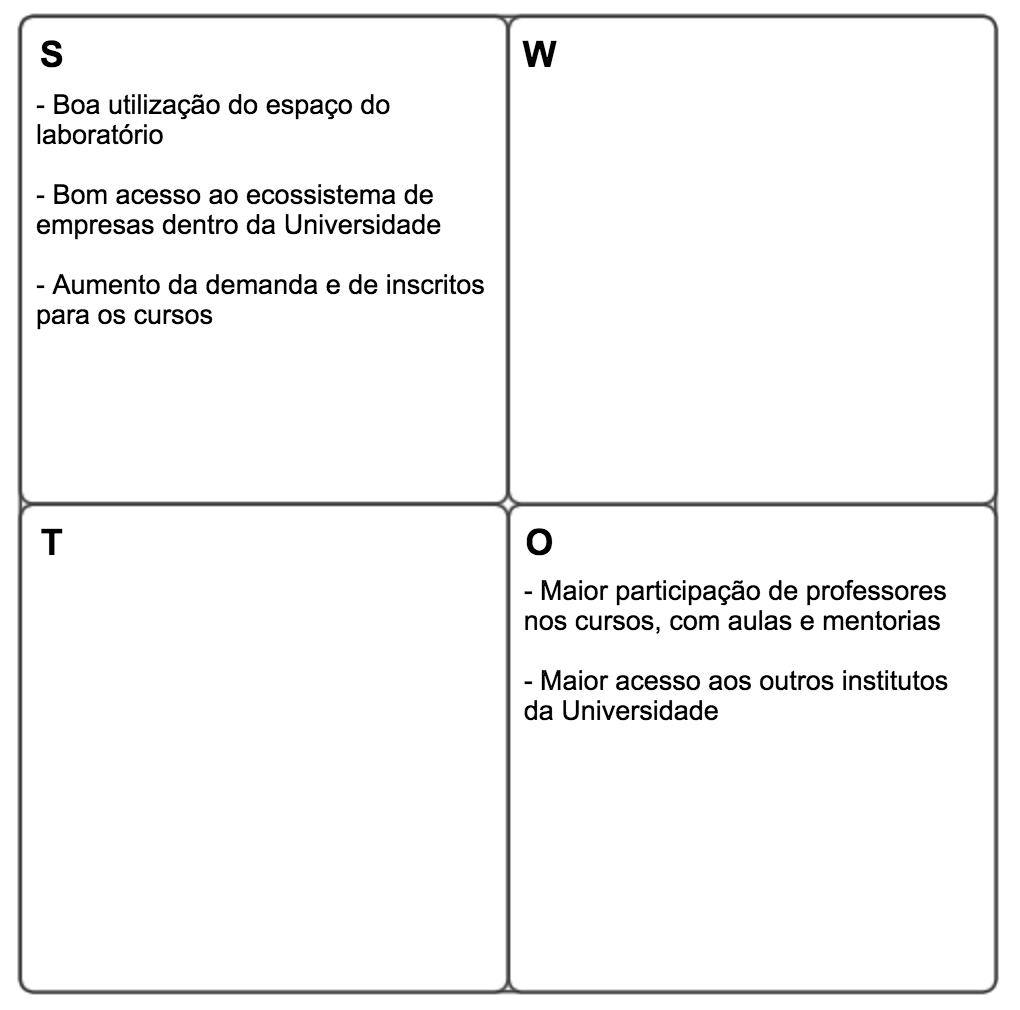
\includegraphics[scale=0.75]{img/samsungswot}}
\label{fig:swotsamsung}
\caption* {Fonte: Elaborado pelo próprio autor}
\end{figure}

\section{PRO}

Para a obtenção dos dados relacionados ao PRO, foram entrevistados o professor Fernando Laurindo - chefe do departamento - e o professor Eduardo Zancul, que possui participação ativa no laboratório Ocean e no InovaLab. 

Em um primeiro momento, a parceria com o Ocean é vista como um projeto de investimento externo aplicado ao departamento e à universidade que surgiu e foi executado com muita rapidez. Entre as conversas iniciais e o final da reforma da área do laboratório foram cerca de 4 meses. Esses fatores são consequência do comprometimento por parte tanto do departamento, que agilizou toda burocracia para permitir a criação do laboratório, quanto por parte da Samsung, que se encarregou e custeou toda construção do laboratório. Esse comprometimento se deu principalmente pela sinergia do projeto Ocean dado ao ecossistema de inovação e empreendedorismo que cresce cada vez mais dentro da universidade e a vontade da Samsung de se aproximar cada vez mais da comunidade estudantil.

Para o professor Eduardo Zancul, existe uma clara conexão estratégica entre o Ocean, o InovaLab e os outros projetos do departamento e para ele, esse foi um dos principais fatores que despertaram na Samsung o interesse de mover o laboratório para dentro da universidade. Foi através do Inovalab que foi feito o primeiro contato com a Samsung, e o NEU colabora ativamente com os cursos intensivos do Ocean, trazendo mentores e palestrantes para auxiliar nos cursos. Dentro desse ecossistema de projetos geridos pelo PRO, o laboratório Ocean representa o elemento tecnológico - em especial dispositivos móveis, realidade virtual, \textit{games} e internet das coisas - e a capacitação técnica para desenvolver projetos nessas frentes, incentivando os projetos que surgem no InovaLab e no NEU. Dessa forma, projetos de inovação podem gerar projetos de empreendedorismo ou pessoas interessadas por inovação podem se engajar por projetos de empreendedorismo com maior facilidade.

O empreendedorismo, em particular, sempre acompanhou a trajetória de alunos da Poli que optaram por abrir a sua própria empresa ao invés de entrarem no mercado de trabalho através do recrutamento de empresas. Não obstante, muitas empresas tiveram o desenvolvimento de seu modelo de negócio realizado em paralelo ao trabalho de graduação de alunos. Por isso a Poli busca sempre oferecer recursos que forneçam a estrutura necessária para os alunos buscarem o seu aprendizado.

À parte da relação com outros projetos, uma das principais discussões sobre o laboratório gira em torno de como utilizá-lo para incentivar as frentes de pesquisa, ensino e extensão baseado nas propostas do laboratório. Atualmente, o laboratório é utilizado por duas disciplinas optativas do departamento, e está liberado para o uso de qualquer disciplina obrigatória, com a única condição de que o formato da aula apresente uma demanda da infraestrutura do laboratório, senão o PRO disponibiliza uma sala de informática com os equipamentos necessários, porém com menor sofisticação do que o Ocean.

Entretanto como ainda está em fase inicial, não houve tempo para os pós-graduandos começarem a utilizar o espaço e iniciar as pesquisas, sendo essa a maior oportunidade de desenvolvimento do laboratório, que segundo os professores acontecerá inevitavelmente, é apenas uma questão de algum aluno se disponibilizar a fazer algo relacionado ao Ocean.

Como parceiro de cogestão do Ocean, o PRO é dono e responsável pelo espaço do laboratório e pode utilizá-lo conforme sua necessidade, incluindo aulas, palestras, seminários, eventos internos e até eventos externos, se houver a oportunidade. Por via de regra, o PRO pode ceder o espaço a eventos ligados a outras universidades ou a entidades sem fins lucrativo. Caso não se enquadre nesses dois casos mencionados o PRO pode alugar o espaço a um baixo custo, de forma a arrecadar recursos para o departamento.

A partir das conversas com os professores, foi criada a seguinte análise:

\begin{figure}[H]
\caption{Análise do Ocean - PRO}
\centerline{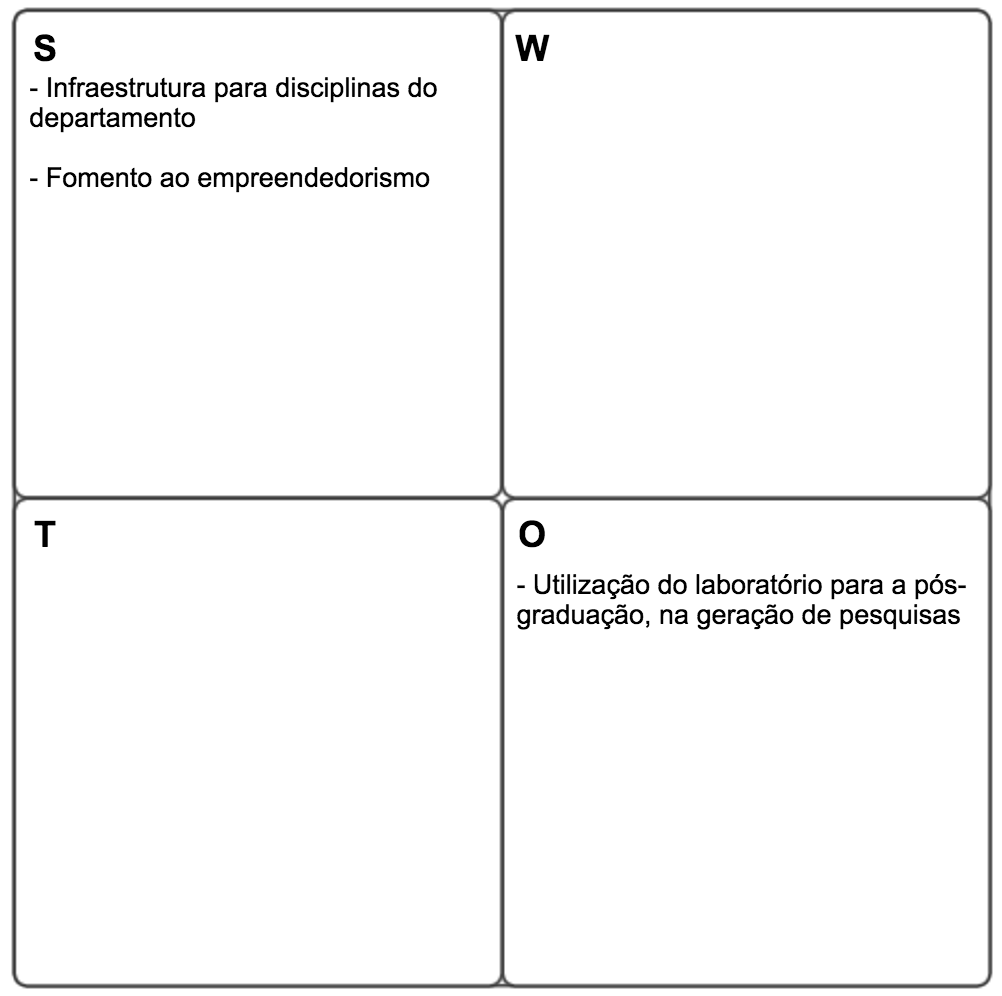
\includegraphics[scale=0.75]{img/proswot}}
\label{fig:swotpro}
\caption* {Fonte: Elaborado pelo próprio autor}
\end{figure}

\section{NEU}

Segundo Juliana Uechi, atual responsável pelo funcionamento do NEU, a presença do Ocean por si só já contribui com o fomento à cultura de empreendedorismo dentro da Universidade, principal objetivo do NEU. Isso porque ainda existe uma carência de motivação pelo empreendedorismo, ainda mais em tempos de crise, a qual encontra no Ocean uma ferramenta gratuita com suporte à pré-aceleração de empresas. 

Atualmente existe uma colaboração ativa entre NEU, PRO e Samsung, principalmente em relação ao atual módulo de curso intensivo do laboratório, que envolve participação de todas as partes. De forma geral, a Samsung é responsável pelo acompanhamento do programa e pela capacitação, e o NEU e o PRO utilizam de suas conexões para trazer mentores às empresas participantes, normalmente ex-alunos que abriram as próprias empresas. Tais colaborações poderiam, segundo Juliana, ir além da participação nos cursos intensivos, porém a agenda de ambas as instituições encontra-se lotada

Em relação à infraestrutura do laboratório, o NEU acredita que o uso do laboratório é subutilizado quando cursos não estão acontecendo. O cenário atual de funcionamento é similar ao de uma biblioteca ou uma sala pró-aluno, onde alunos vão com tarefas individuais ou materiais de estudo, o que é de certa forma redundante pois já há uma biblioteca no departamento. Como uma frente de desenvolvimento e empreendedorismo, poderia haver mais espaço para \textit{coworking} e atividades colaborativas dentro do laboratório. O ideal seria que fosse uma sala que gerasse valor através da discussão, não da absorção individual, que é igualmente importante, mas a biblioteca seria um lugar mais adequado para esse tipo de atividade.

Por fim, é ressaltado a sinergia entre empresas que colaboram com o fomento à cultura de empreendedorismo, considerando que por mais que compartilhem o relacionamento com \textit{startups} via pré-aceleração, os alunos precisam ser motivados através de métodos diferentes. E pensando sempre no aluno e nas suas futuras empresas, um ambiente com diversas instituições de fomento ao empreendedorismo e aceleração, evita a entrada na universidade de instituições não-gratuitas, seja através de inscrição nos cursos ou via equity das empresas.

A partir da conversa com a Juliana, foi obtida a seguinte análise:

\begin{figure}[H]
\caption{Análise do Ocean - NEU}
\centerline{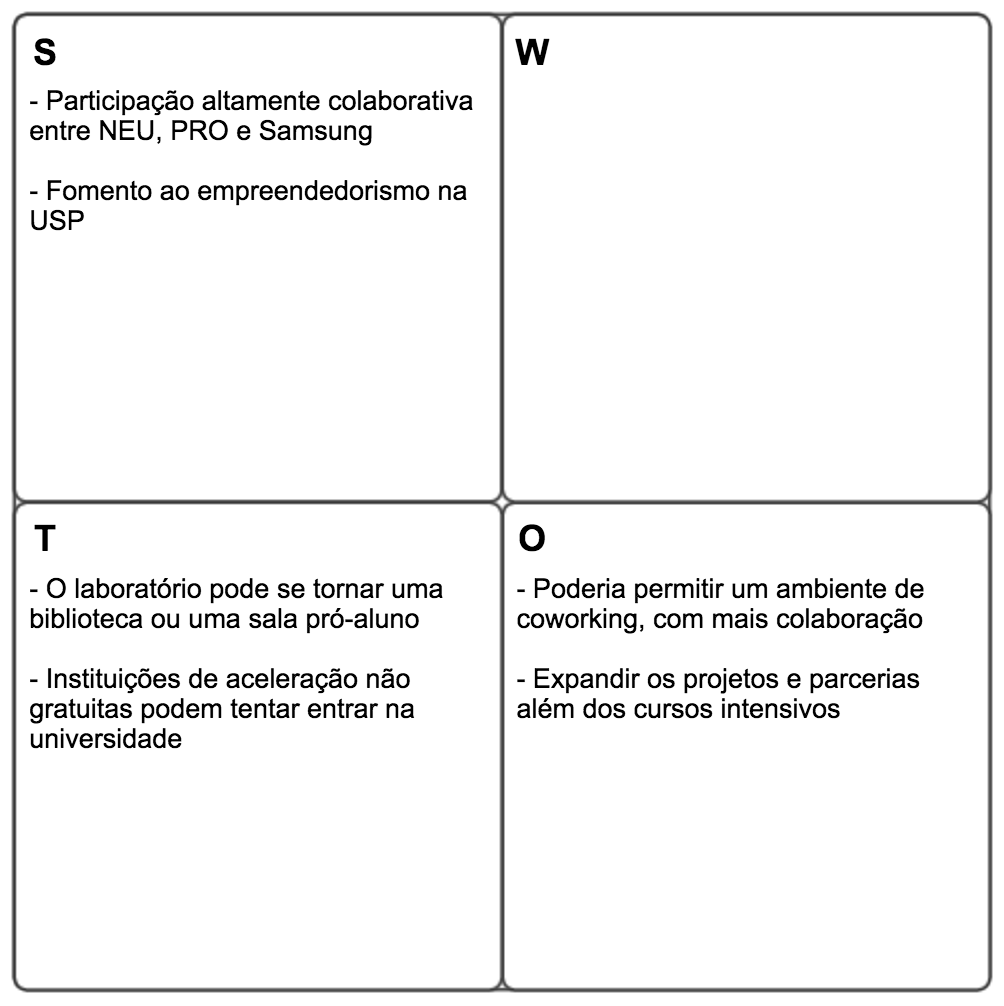
\includegraphics[scale=0.75]{img/neuswot}}
\label{fig:swotneu}
\caption* {Fonte: Elaborado pelo próprio autor}
\end{figure}

\section{Alunos}

De forma a obter as percepções dos alunos diante do laboratório, foram realizadas entrevistas com dez pessoas, entre alunos que frequentavam o laboratório no momento da entrevista e membros do centro acadêmico. Primeiramente, o que se observou em todas as respostas foi uma comparação direta entre o laboratório e duas estruturas do PRO: a biblioteca e a sala de informática. 

A biblioteca atual do departamento funciona de segunda à sexta-feira, das 8h00 até as 18h00, e possui 8 salas para grupos de 4 pessoas, e entre mesas compartilhadas e individuais, possui capacidade para cerca de mais 20 alunos. Parte da biblioteca está interditada por problemas de infraestrutura, que não têm previsão de serem resolvidos, e por ora deixam de abrigar cerca de 30 alunos que poderiam ocupar esse espaço. Para os alunos de engenharia de produção, o laboratório Ocean foi extremamente bem vindo, pois cobre diversos problemas da biblioteca, como o acesso a um wifi de maior qualidade, funcionamento após as 18h e lugares disponíveis frente às salas da biblioteca cheias. Não obstante, o laboratório ainda possibilita utilizar os monitores com os próprios notebooks, que segundo os alunos são mais utilizados que os notebooks da Samsung.

A sala de informática se localiza em uma antiga sala de aula do departamento, e é utilizada em aulas que demandam o uso de algum \textit{software} ou é necessário a prática de programação, como \enquote{Controle e Automação}, \enquote{Modelagem e Simulação de Sistemas de Produção}, \enquote{Sistemas de Informação}. Entretanto, segundo alguns alunos, os equipamentos muitas vezes deixam a desejar e atrapalham no acompanhamento das disciplinas. Dada a qualidade dos equipamentos, os alunos prefeririam utilizar os computadores do laboratório para obter maior fluidez nas aulas. Não só, os alunos acreditam que mais aulas poderiam ser informatizadas, como \enquote{Pesquisa Operacional}, \enquote{Logística} e \enquote{Finanças}, ressaltando que apesar de a prática dessas disciplinas envolverem um uso intensivo de softwares, como Excel e Lingo/Lindo, parte das aulas ainda utiliza retroprojetores para explicações e exercícios. Portanto, os alunos acreditam que o laboratório pode contribuir com a melhoria da dinâmica das aulas.

De forma geral, todos avaliam o laboratório positivamente, porém ressaltaram alguns problemas com a sua utilização. Um dos problemas diz respeito ao processo de utilização do laboratório, pois não há políticas muito claras sobre o uso ou indicações sobre o que é ou não é permitido na sala, principalmente sobre a utilização dos notebooks ou monitores. Também não está claro a quem perguntar para tirar dúvidas, pois não há um monitor na sala. Outro ponto levantado é a falta de algum lugar para consultar se a sala estará disponível para uso com antecedência, relevante para alunos poderem se programar se utilizarão o laboratório ou terão que ir para outro lugar. Por fim, alguns alunos dizem não saber o conteúdo ou o tema dos cursos dados pelo programa Ocean, e têm sua percepção através do espaço físico do laboratório apenas. 

A partir das conversas com os alunos, foi desenhada a seguinte análise:

\begin{figure}[H]
\caption{Análise do Ocean - Alunos}
\centerline{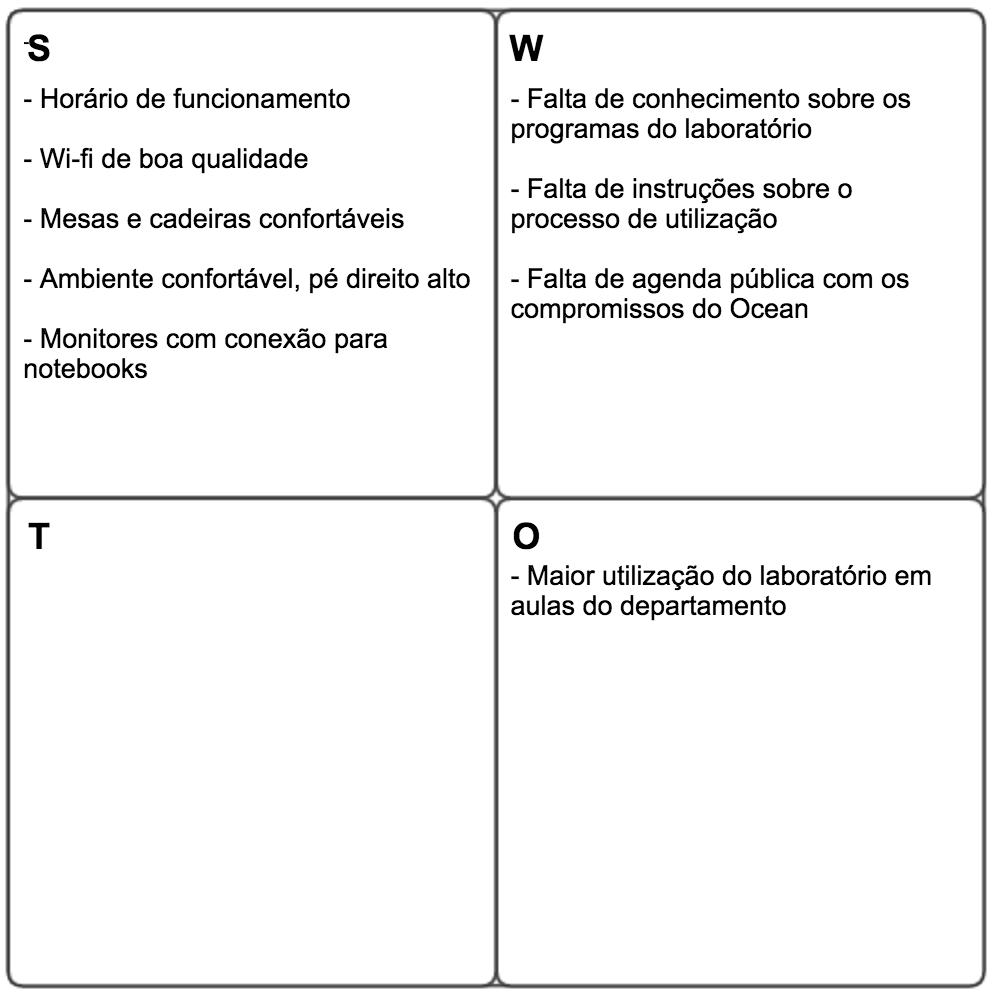
\includegraphics[scale=0.75]{img/alunosswot}}
\label{fig:swotalunos}
\caption* {Fonte: Elaborado pelo próprio autor}
\end{figure}

\section{Cursistas}

A análise dos cursistas é segmentada devido aos dois tipos de cursos dados pelo laboratório e o tipo de material a ser analisado para cada. Para os alunos de cursos básicos, foi utilizada a metodologia de \citeonline{bardin} para analisar os questionários de respostas, ao passo que com os alunos de cursos intensivos foram realizadas entrevistas semi-estruturadas.

\subsection{Cursos Básicos}

Em relação aos cursistas dos cursos básicos, utilizamos o software desenvolvido pelo autor para mapear as palavras com maior recorrência nas respostas dos questionários para cursos básicos, para as seguintes perguntas:

\begin{itemize}
\item O que mais o motivou nesse curso?
\item O que você acha que pode ser melhorado?
\item Qual tema você gostaria que fosse abordado num próximo curso?
\end{itemize}

Como forma de simplificação, foram utilizados como nomenclatura de cada questão os termos \enquote{motivação}, \enquote{melhorias} e \enquote{novidades}, respectivamente. Em seguida, foi aplicada a metodologia de \citeonline{bardin} para as respostas de cada uma.

\subsubsection*{Pré-exploração do material}

A pré-exploração segue o mesmo modelo para todas as questões, devido aos seguintes motivos:

\begin{description}
\item[Modelo único de coleta] O instrumento de coleta de dados utilizado nas pesquisas foi o mesmo questionário reutilizado nos últimos 2 anos. Dado que no momento de preenchimento os cursistas acabaram de realizar os cursos, a percepção deles diante do conteúdo passado está bem fresca, e a contribuição também acaba sendo maior com uma taxa maior de respostas. Isso permitiu que o autor minimizasse a possibilidade de encontrar poucos dados ou dados inconsistentes com a realidade apresentada no curso.
\item[Perguntas sequenciais com o mesmo formato] As perguntas qualitativas no final do questionário são bastante diretas e fáceis de serem respondidas. O objetivo de cada questão pode ser traduzido pela própria nomenclatura previamente estabelecida: identificar a motivação dos cursistas que optaram por {gastar} cerca de 3 horas em um curso de capacitação, identificar melhorias dentro do próprio curso para melhorar a sua qualidade de forma geral, e estar sempre atualizado para identificar a sinergia entre esse curso e outros temas de interesse dos cursistas. O formato das perguntas permitiu uma análise não exaustiva de dados pois as respostas apresentavam algumas poucas linhas, e a informação presente é suficiente para atender as necessidades da Samsung.
\item[Respostas consolidadas em um mesmo lugar] Todas as respostas foram consolidadas em planilhas digitais, de tal forma que cada resposta corresponde a uma linha, e cada pergunta é uma coluna. Esse formato simplificou a leitura flutuante realizada sobre as respostas, pois um simples \textit{scroll} na tela já traz um novo set de respostas, sem haver muito desgaste mental do autor.
\end{description}

Conforme foi ressaltado, a leitura flutuante foi o principal elemento da pré-exploração do material, pois permitiu identificar o tamanho das respostas (curtas), a variedade das respostas (baixa) e a consequente pré-aprovação da possibilidade de analisá-las e categorizá-las posteriormente. Embora sejam só características relativas observas pelo autor, elas representam a inferência ilustrada por \citeonline{bardin} como pontos de partida ou hipóteses para as próximas etapas.

\subsubsection*{Definição das unidades de análise}

Embora o autor já tivesse ideia da convergência das respostas para certos temas devido às observações obtidas na fase de pré-exploração, não saberia ainda descrever quais seriam os temas principais, e muito menos quantificá-los por número de incidências. Portanto, de forma a tentar atribuir as principais categorias, foi decidido analisar o número de incidências de cada palavra em todas as respostas, por se tratarem de textos curtos e informais.

Após uma análise inicial, observou-se que muitas palavras tinham sinergia entre si e apresentavam-se dentro de um mesmo contexto. Portanto também foram mapeadas todas as palavras que aparecem em uma mesma frase que outro palavra. Dessa forma é possível observar as palavras que aparecem em um mesmo contexto, e logo, possuem bastante sinergia entre si.

Foi considerado como premissa que todas as palavras de cada resposta não se repetem na mesma resposta - com exceção de palavras auxiliares, como artigos e pronomes - de tal forma que seria possível atribuir a linha de origem de cada palavra sem repetições.

\subsubsection*{Tratamento dos dados}

De forma a configurar o \textit{software} a trabalhar em cima das respostas, foi feita uma extração dos dados da planilha no \textit{software} \textit{Numbers} em um MacBook para o formato CSV, que é um arquivo de texto puro com quebras de linha e separação por vírgulas. Como o arquivo original, cada linha corresponde a uma resposta e cada elemento entre vírgulas corresponde a uma pergunta. Portanto para cada pergunta a ser analisada, são percorridas todas as linhas e só analisados os elementos correspondentes.

Por se tratarem de todas as palavras da língua portuguesa, foi feito um trabalho manual e iterativo de descartar todas as palavras que não agregariam valor semântico esperado à frase, como pronomes, artigos, verbos auxiliares, conjunções e preposições. Foi uma opção não realizar uma integração com algum software ou \textit{Web API} de Língua Portuguesa pela necessidade e esforço em garantir a confiabilidade do mesmo, portanto a partir do próprio conhecimento do idioma foram feitas iterações e remoções de palavras indesejadas.

Também foram eliminadas as palavras relativas à \enquote{curso} e \enquote{aula}, pois todas as perguntas são direcionadas a como melhorar, motivar ou trazer novas coisas para o curso e para a aula, portanto foram consideradas redundantes para a análise.

Outro tratamento realizado foi a remoção de espaços em excesso, pontuações e o emprego das aspas, pois estes atrapalhavam a contagem de palavras.

A partir dos tratamentos descritos e de outros específicos a cada questão, foi possível elaborar uma tabela como \textit{output} do \textit{software} utilizado. A tabela representa uma contagem das principais palavras presentes nas respostas, acompanhadas de outras que aparecem em um mesmo contexto, e de um exemplo de respostas para ilustrar o uso das palavras de forma conjunta. O exemplo é obtido randomicamente através de uma busca por respostas que apresentem ambas as palavras. Para isso, foram adotadas algumas constantes para aplicação no software:

\begin{itemize}
\item Número mínimo de incidências para ser considerado na tabela: 1\% do número de respostas
\item Número de palavras com sinergia que são exibidas: 3
\end{itemize}

Esses números foram definidos posteriormente, pois foram feitos alguns testes para identificar até onde poderia ser filtrado os dados para não perder nenhuma informação relevante. Essas constantes se apresentaram boas tanto de forma ilustrativa para o trabalho quanto para a categorização posteriormente feita das palavras.

\subsubsection*{1\textsuperscript{a} Questão: \textit{Motivação} - Tratamento dos dados }

Novamente, como não há integração com um dicionário de Língua Portuguesa, foi possível de fazer agrupamentos de palavras que se encontravam em um mesmo contexto, comprovado pelas sinergia com as mesmas palavras ou similares. 

Foi possível agrupar posteriormente palavras que se apresentavam em diferentes flexões gramaticais de número, como: 

\begin{itemize}
\item \enquote{conhecimento} e \enquote{conhecimentos}
\item \enquote{tecnologia} e \enquote{tecnologias} 
\item \enquote{novas} e \enquote{nova} 
\item \enquote{ferramenta} e \enquote{ferramentas} 
\item \enquote{novos} e \enquote{novo} 
\item \enquote{apps} e \enquote{app}
\item \enquote{aplicativos} e \enquote{aplicativo}
\end{itemize}

Também foram agrupadas palavras com flexões gramaticais de gênero:

\begin{itemize}
\item \enquote{novas} e \enquote{novos}
\end{itemize}

Por fim, palavras com mesmo nível semântico:

\begin{itemize}
\item \enquote{app} e \enquote{aplicativo}
\item \enquote{instrutor} e \enquote{professor}
\end{itemize}

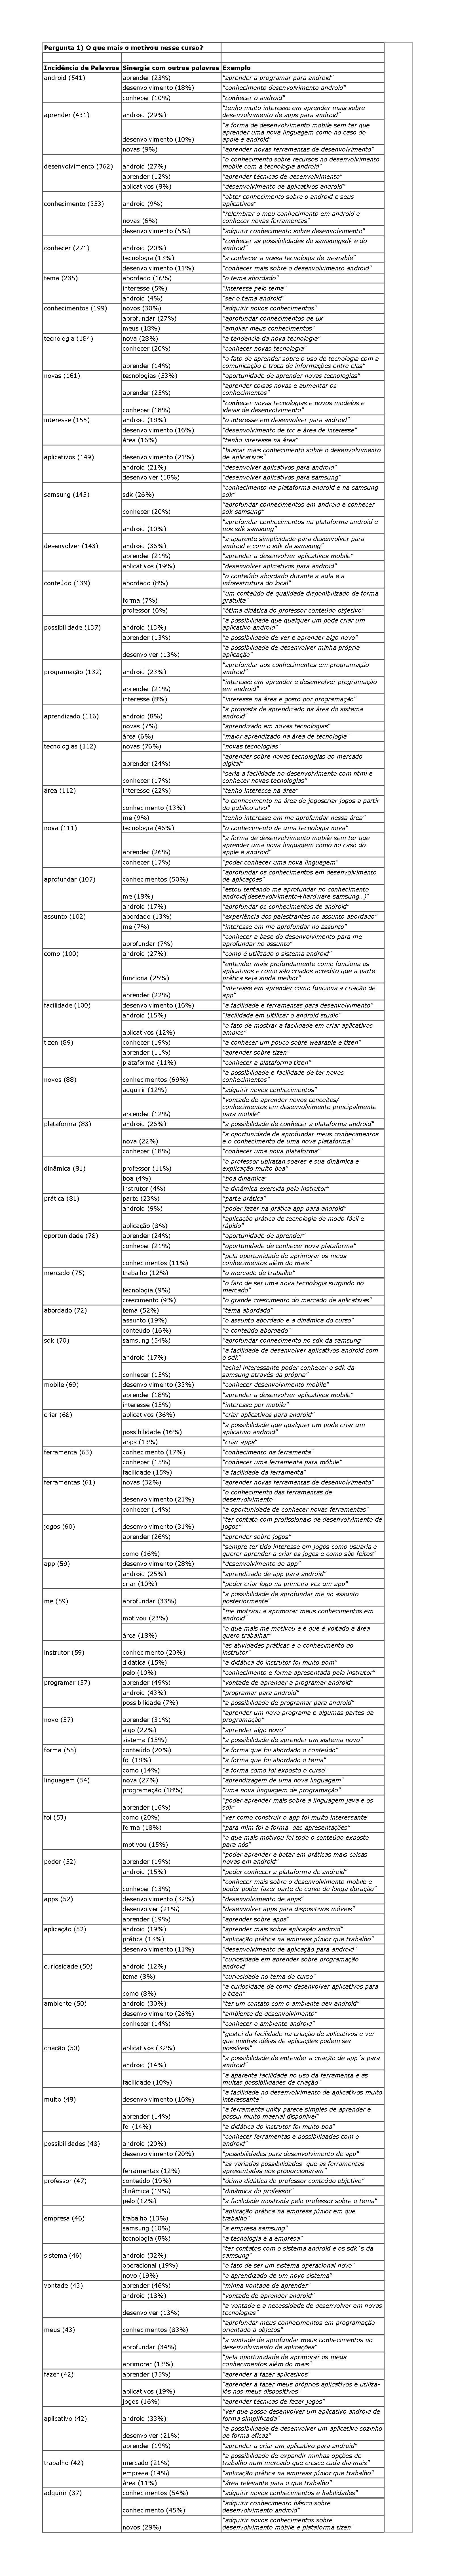
\includepdf[pages=-, pagecommand={}]{Pergunta1.pdf}

\subsubsection*{1\textsuperscript{a} Questão: \textit{Motivação} - Categorização e sub-categorização }

Após analisar a incidência de palavras, foi possível observar a partir dos exemplos uma ambiguidade promovidos pela pergunta em questão. A interpretação correta dessa pergunta seria \enquote{quais foram os pontos do curso que você achou mais interessante / relevante?}, porém a maior parte das respostas aparentemente a interpretou como \enquote{o que o motivou a fazer o curso?}. Isso gerou uma séria de respostas relacionadas ao próprio tema do curso, como \enquote{interesse por desenvolvimento android e SDK da samsung}. Dado que o tema mais recorrente de apresentação do curso chama-se \enquote{Introdução ao Desenvolvimento de Aplicativos Android \& Samsung SDK}, acaba-se por ter respostas redundantes. Também ocorreram respostas inerentes ao contexto de mercado de trabalho envolvendo programação, o que também foge do objetivo proposto por essa pergunta. Foi passado para a Samsung uma proposta de reformulação dessa pergunta, baseada em como deseja-se utilizar essa informação posteriormente.

Entretanto, ainda foi possível extrair algumas informações a respeito de pontos elogiados do curso, como:

\begin{itemize}
\item A ocorrência de \enquote{professor} e \enquote{dinâmica} indicaram a aceitação pelos alunos do modelo proposto pelo curso, e elencaram estes como um fator motivador.
\item A palavra \enquote{prática} indica que os alunos gostaram da parte prática dos cursos, que indiretamente deve contribuir com a dinâmica elogiada no item anterior.
\end{itemize}

A partir desses pontos, foram extraídas as seguintes categorias para a questão \enquote{O que mais o motivou nesse curso?}:

\begin{figure}[H]
\caption{Categorias para a questão 1}
\centerline{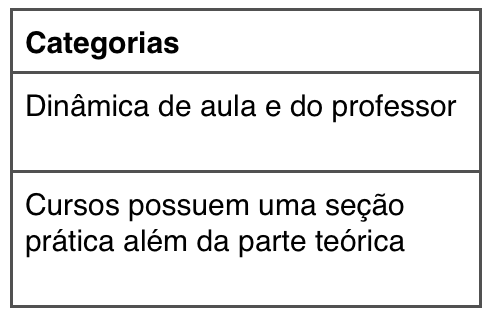
\includegraphics[scale=0.75]{img/categoriasmotivacao}}
\label{fig:categoriasmotivacao}
\caption* {Fonte: Elaborado pelo próprio autor}
\end{figure}

\pagebreak
\subsubsection*{2\textsuperscript{a} Questão: \textit{Melhorias} - Tratamento dos dados }

Em relação à flexão gramatical de número e gênero e semântica, foram agrupadas as seguintes palavras

\begin{itemize}
\item \enquote{práticas}, \enquote{práticos}, \enquote{prático} e \enquote{prática}
\item \enquote{professor}, \enquote{instrutor}, \enquote{instrutores} e \enquote{professores}
\item \enquote{conhecimento} e \enquote{conhecimentos}
\item \enquote{app}, \enquote{apps}, \enquote{aplicativo} e \enquote{aplicativos}
\end{itemize}

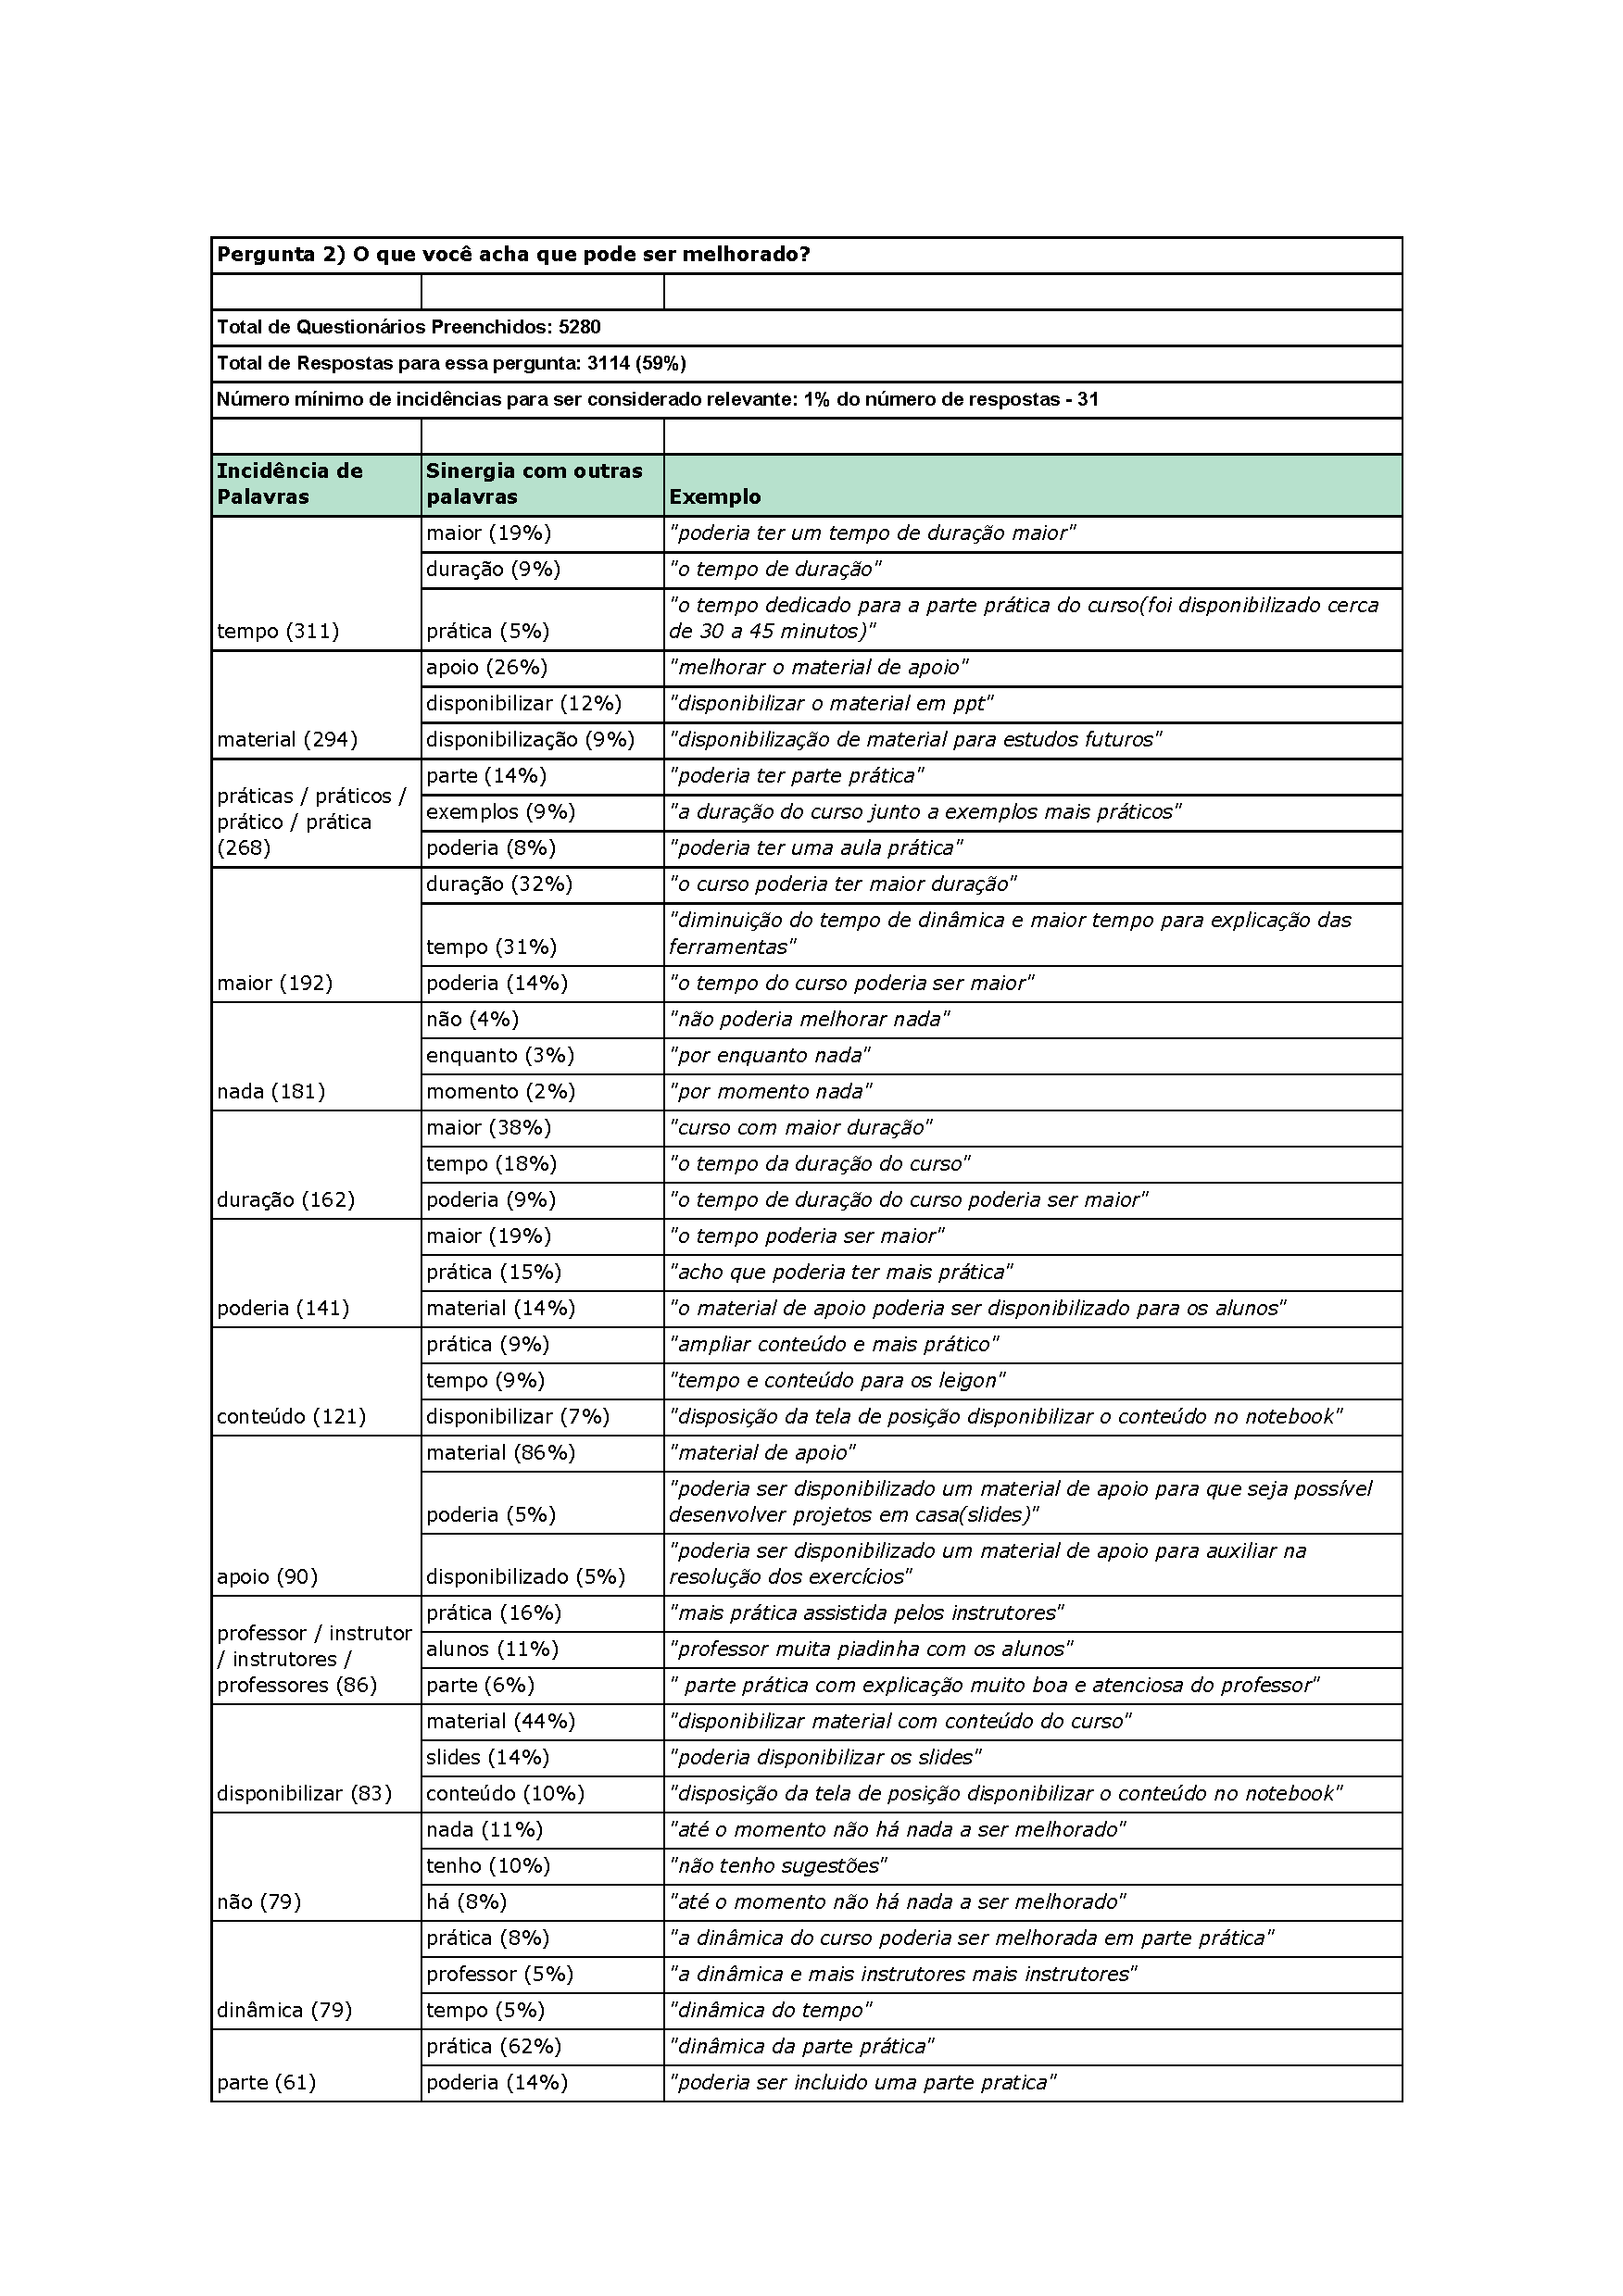
\includepdf[pages=-, pagecommand={}]{Pergunta2.pdf}

\subsubsection*{2\textsuperscript{a} Questão: \textit{Melhorias} - Categorização e sub-categorização }

Diferentemente da questão anterior, esse item é compreendido muito melhor pelos alunos, e as respostas tornam-se muito mais objetivas. A recorrência já mostra de imediato três pontos a serem melhorados, a duração do curso, problemas com o material de apoio e a inclusão de mais modalidades práticas dentro da aula. Esses problemas, de forma conjunta, correspondem a cerca de 40\% das respostas analisadas.

A duração do curso se mostra um grande problema, se mostrando incidente através das palavras \enquote{tempo}, \enquote{duração} e \enquote{carga horária}, essa última com as duas palavras aparecendo na tabela.

Os problemas com o material de apoio também se mostra recorrente através da expressão \enquote{material de apoio}, \enquote{conteúdo}, \enquote{slides}, \enquote{slides} e \enquote{apresentação}. A maior parte se associa com as palavras \enquote{disponibilizar} e \enquote{disponibilização}, indicando que o material utilizado não é entregue para os alunos.

A recorrência de termos ligados à prática indica que há uma necessidade de aumentar a parte prática no programa diante da teórica. Aliada essa informação à questão da carga horária, deve ser desejável que se for possível aumentar o tempo de curso, que ele aumente em termos práticos e não teóricos.

Em menor volume (menos de 5\% cada), aparecem pontos como maior flexibilização do horário ou disponibilidade de horários, através das palavra \enquote{horário} e \enquote{dias}, e problemas com equipamentos no laboratório.

A partir desses pontos, foram extraídas as seguintes categorias para a questão \enquote{O que você acha que pode ser melhorado?}:

\begin{figure}[H]
\caption{Categorias para a questão 2}
\centerline{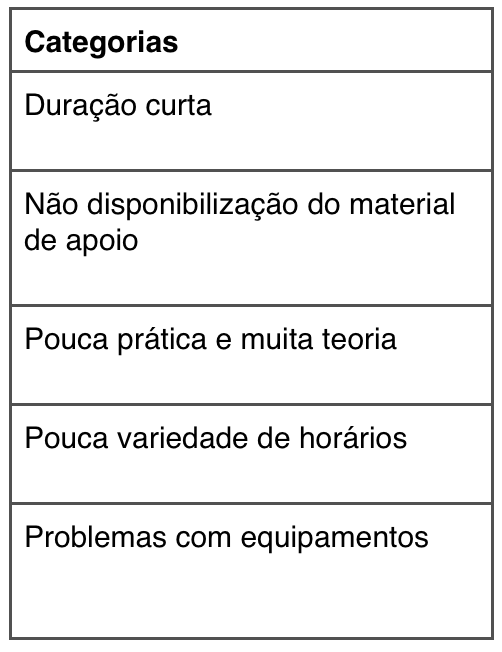
\includegraphics[scale=0.75]{img/categoriasmelhorias}}
\label{fig:categoriasmelhorias}
\caption* {Fonte: Elaborado pelo próprio autor}
\end{figure}

\subsubsection*{3\textsuperscript{a} Questão: \textit{Novidades} - Tratamento dos dados }

Em relação à flexão gramatical de número e gênero e semântica, foram agrupadas as seguintes palavras

\begin{itemize}
\item \enquote{jogos}, \enquote{jogo}, \enquote{game} e \enquote{games}
\item \enquote{aprofundar} e \enquote{aprofundamento}
\item \enquote{práticas}, \enquote{práticos}, \enquote{prático} e \enquote{prática}
\item \enquote{app}, \enquote{apps}, \enquote{aplicativo} e {aplicativos}
\end{itemize}

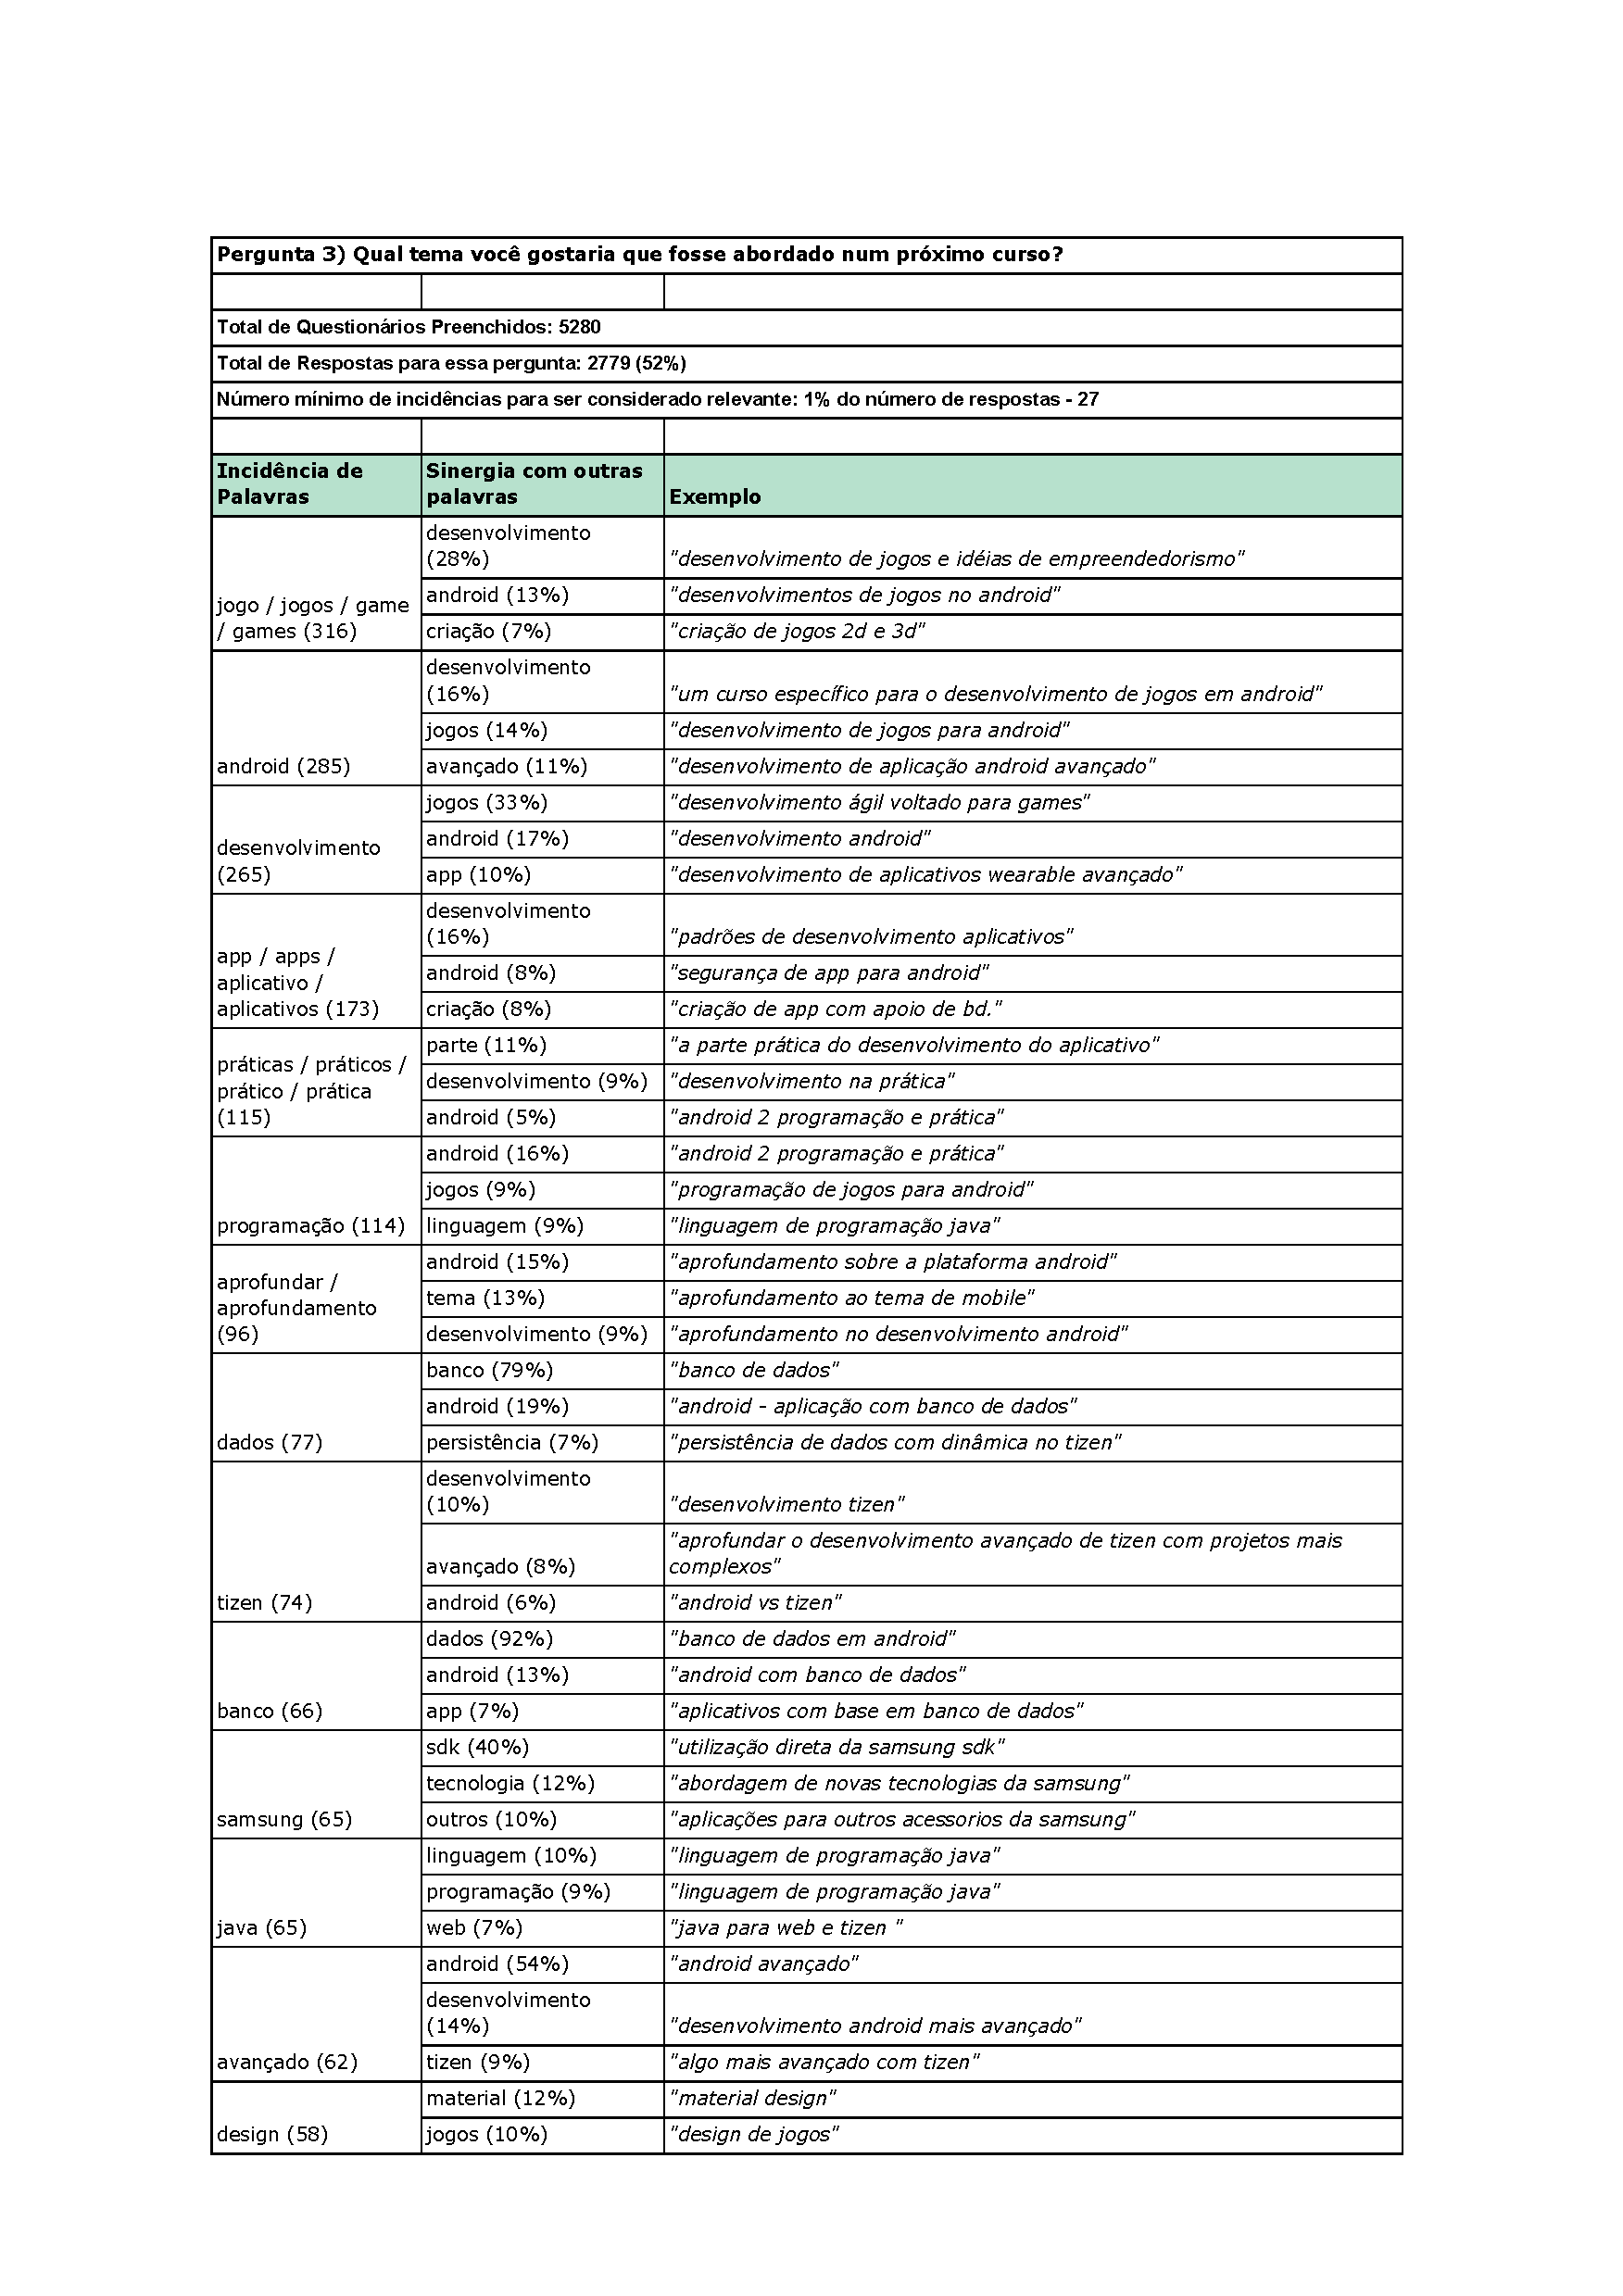
\includepdf[pages=-, pagecommand={}]{Pergunta3.pdf}

\subsubsection*{3\textsuperscript{a} Questão: \textit{Novidades} - Categorização e sub-categorização }

Em primeira instância, é possível visualizar uma grande demanda de alunos por aulas específicas para o desenvolvimento de jogos. É de grande relevância que esta questão é a de escopo mais aberto das três, portanto a grande recorrência do termo \enquote{jogo} nesse contexto é bastante relevante. Além de jogos, existe uma demanda pela aplicação de android em outros casos de uso, como aplicativos ou uma exploração mais avançada do sistema operacional. 

Em menor volume porém com uma maior gama de opções, existe uma demanda por uma exploração de bancos de dados, tizen, maior exploração do sdk da samsung e outras tecnologias, linguagem de desenvolvimento java, design e user experience, desenvolvimento web, web services, e unity. 

A partir desses pontos, foram extraídas as seguintes categorias para a questão \enquote{Qual tema você gostaria que fosse abordado num próximo curso?} :

\begin{figure}[H]
\caption{Categorias para a questão 3}
\centerline{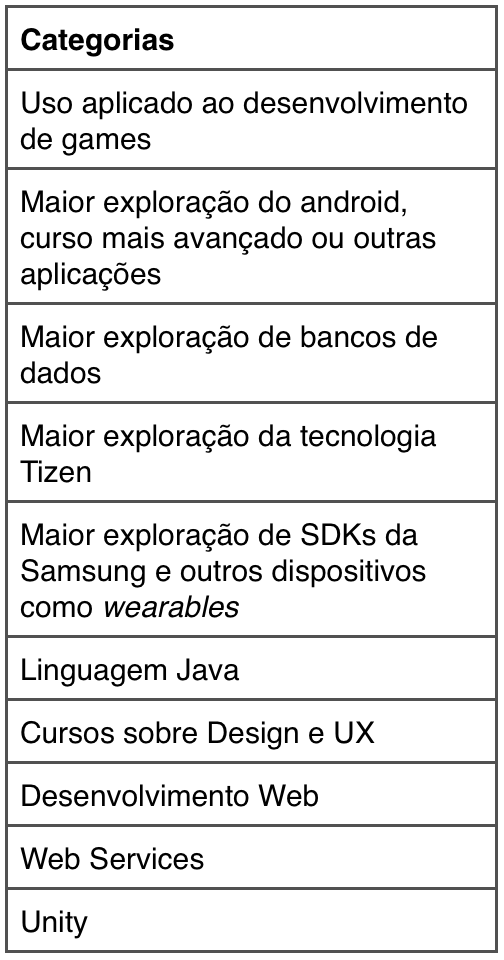
\includegraphics[scale=0.75]{img/categoriasnovidades}}
\label{fig:categoriasnovidades}
\caption* {Fonte: Elaborado pelo próprio autor}
\end{figure}

A partir das categorias obtidas para todas as questões, foi definida a seguinte análise:

\begin{figure}[h]
\caption{Análise do Ocean - Cursistas - Cursos Básicos}
\centerline{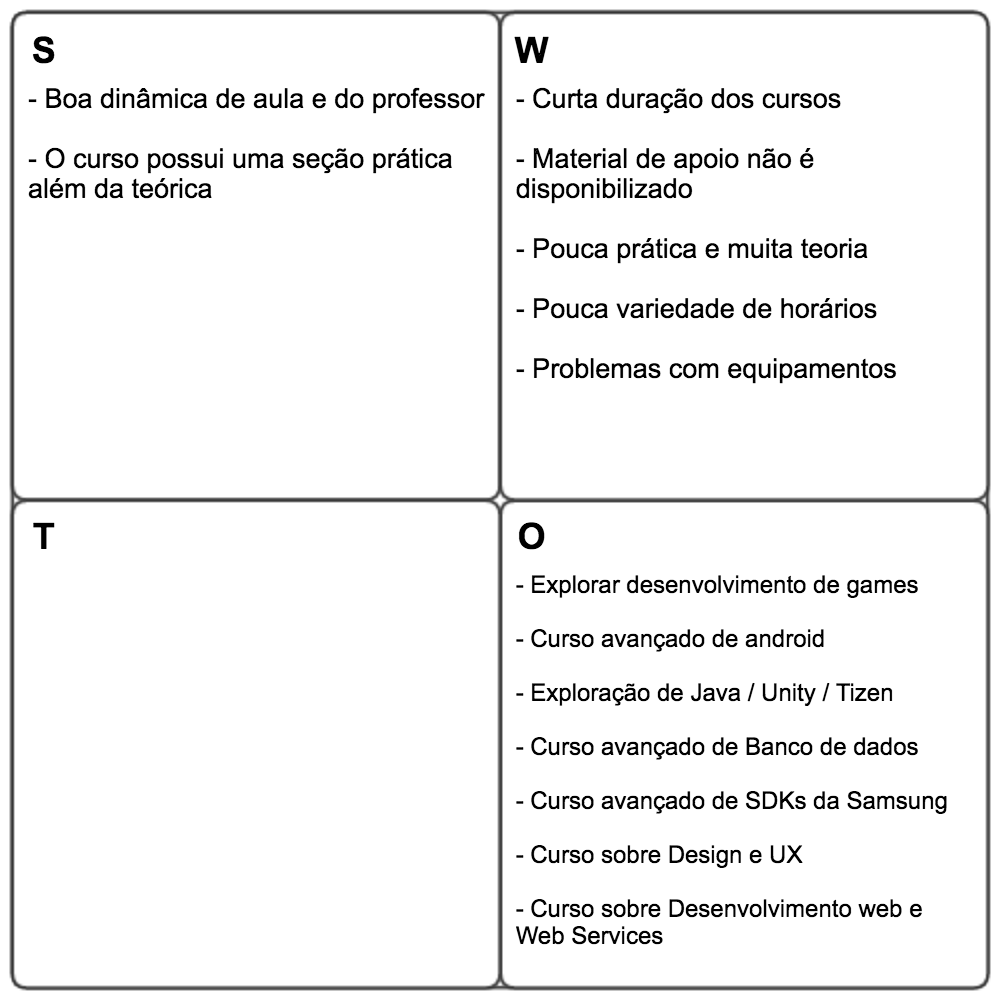
\includegraphics[scale=0.75]{img/cursosbasicosswot}}
\label{fig:swotcursosbasicos}
\caption* {Fonte: Elaborado pelo próprio autor}
\end{figure}

\subsection{Cursos Intensivos}

Para a análise dos cursos intensivos, foram feitas entrevistas com os grupos participantes da edição atual do módulo de pré-aceleração do programa Ocean. As entrevistas foram realizadas em um dia de mentoria, considerado mais tranquilo para a conversa com todos os grupos presentes.

As conversas com os cursistas foram muito produtivas e os mesmos foram extremamente atenciosos, em primeira instância porque já tinham sido avisados das entrevistas naquele dia, e depois porque eles têm bastante orgulho das suas ideias e gostam muito de falar sobre elas e receber \textit{feedbacks}. Essas conversas foram bastante apreciadas pelo autor pois foi importante para quebrar alguns conceitos que subconscientemente já tinha estabelecido:

\begin{description}
\item[Os cursistas serão alunos de graduação ou recém-formados] 

Embora alguns grupos fossem de alunos em graduação ou com graduação há menos de 2 anos, alguns grupos eram constituídos de pessoas com bastante experiência no mercado de trabalho, incluindo um grupo que o líder é um senhor com mais de 40 anos de experiência em gestão de empresas. Também há alunos de mestrado e pessoas com mais experência com \textit{startups} e as novas tecnologias.

\item[Os cursistas dedicam-se ao projeto em paralelo a um emprego fixo] 

Muitas das pessoas que participam do programa estão se dedicando praticamente todo tempo delas para esse projeto, abrindo mão dos antigos empregos para focar completamente nele. Em especial um casal de Brasília vem para São Paulo e volta toda semana para acompanhar as aulas do curso. Segundo eles todo esforço vai valer a pena para poderem lançar o produto deles, de cunho sócio-ambiental, e a gratuidade do programa já compensa pelo que pagariam por um curso de mesma qualidade em Brasília.

\end{description}

Em comum a todos os grupos, foi possível observar a vontade que eles têm de fazer o produto ser bem-sucedido e a atenção com que escutam e recebem os \textit{feedbacks} dos mentores. O reflexo dessa dedicação se dá na avaliação positiva em relação à intensidade do curso e aos modelos de \textit{checkpoint} semanais realizados pelo programa, que consideram \enquote{puxados}  porém necessários para forçar o grupo a ter agilidade em relação a mudanças e obtenção de respostas em relação ao produto. Não obstante, ainda mostra que o programa Ocean realmente está comprometido com os projetos a serem acelerados.

De acordo com o cronograma do programa Ocean, os grupos só trabalharam até o momento a parte de \textit{Customer Discovery}, entretanto todos ficaram muito satisfeitos com essa primeira parte do curso, exaltando a excelente qualidade do trabalho da aceleradora Baita, que possui uma parceria com o programa Ocean para orientar com maestria esse tópico. A qualidade dos executivos da Baita foi ressaltada inclusive pelos membros mais experiente dos grupos, que consideraram-os como os melhores professores / mentores que já tiveram, mesmo participando de programas de aceleração pagos.

Mesmo com grande satisfação dos cursistas, algumas questões foram levantadas, como a ineficiência de palestras de 3 horas, pois consideram que esse tipo de modalidade é uma transmissão de conhecimento menos eficiente do que através de conversas diretas com os grupos, onde o aprendizado poderia ser mais direcionado. Também foi ressaltado que havia uma diferença considerável entre o estado de maturidade dos produtos de cada grupo, o que atrapalha um pouco a definição de expectativas para os grupos por parte dos avaliadores. A \textit{gamificação} foi outro fator mencionado que, embora não seja um problema em seu núcleo, acaba sendo impactada por alguns fatores, como a diferença de maturidade do produto explicada anteriormente e pela diferença natural do modelo de negócio entre os produtos. Durante o programa, os grupos deveriam competir pelo número de entrevistas a serem realizadas com o público-alvo. Grupos com o produto em um estado mais maduro conseguiam modelar um questionário e onde encontrar o público alvo com mais facilidade do que grupos com o produto em um estado menos maduro, assim como produtos B2B tem uma maior dificuldade de conseguir entrevistas do que os produtos B2C. 

Por fim, acredita-se que a Samsung poderia explorar mais a questão de inovações e tendências tecnológicas para inspirar os cursistas a melhorar a tecnologia de seus produtos. Houveram palestras relacionadas ao tema, porém aparentemente elas rodaram muito em torno de produtos da empresa de forma não natural, fazendo com que parecesse que fosse uma propaganda direta dos produtos. A mesma informação poderia ser passada ao explorar os problemas reais enfrentados pelos usuários e pelo mercado e aí sim mostrar como a Samsung criou soluções para esses problemas. Um dos modelos citados como exemplos de palestras e discussões sobre novas tecnologias como \textit{wearables} e IOT foi o \textit{International Symposium on Consumer Electronics} (ISCE).

A partir das conversas com os cursistas, foi obtida a seguinte análise:

\begin{figure}[H]
\caption{Análise do Ocean - Cursistas - Cursos Intensivos}
\centerline{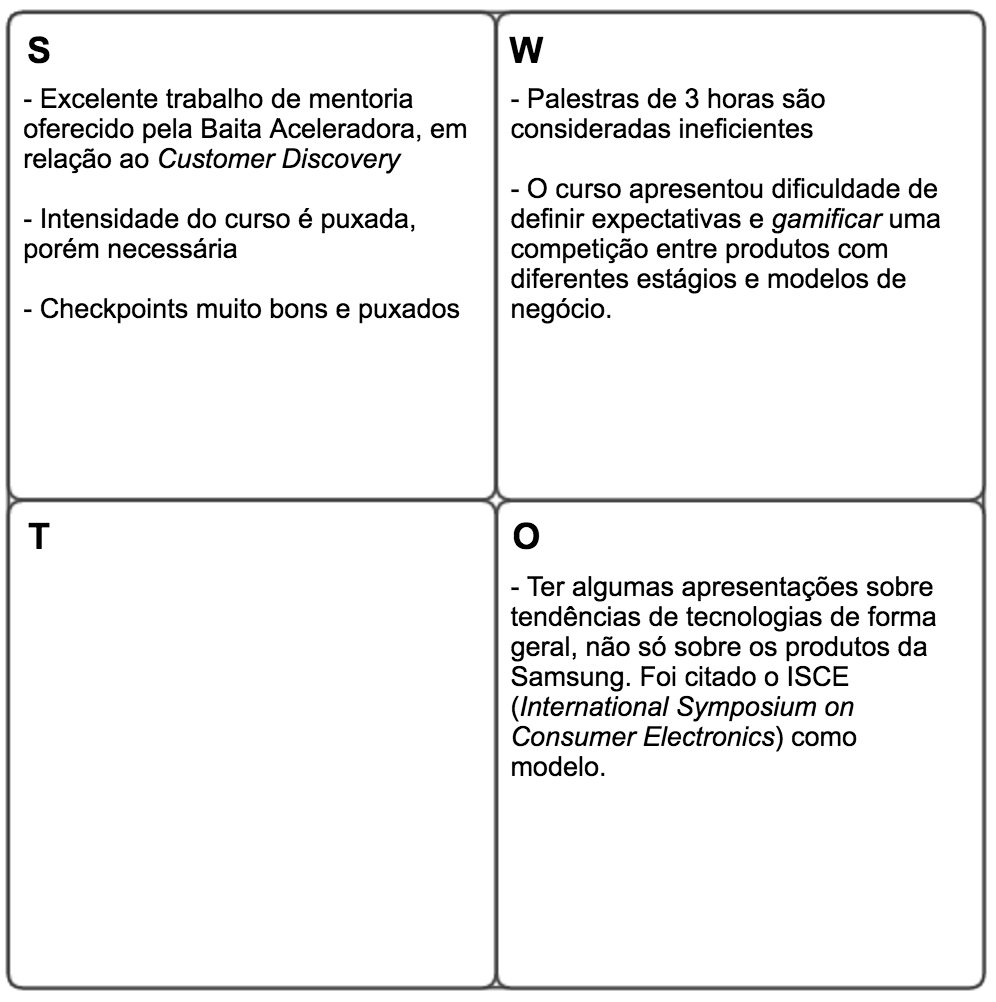
\includegraphics[scale=0.75]{img/cursosintensivosswot}}
\label{fig:swotcursistasintensivos}
\caption* {Fonte: Elaborado pelo próprio autor}
\end{figure}

\subsection{Análise Geral}

Após conversar e analisar todos os \textit{stakeholders}, é possível observar que todos estão muitos satisfeitos com o Laboratório Ocean em seu estado atual, principalmente por ser um projeto em fase inicial, o que evidencia muito as melhorias diante do estado anterior no qual o laboratório não estava presente. Acredita-se que com o passar do tempo e com as interações entre os diferentes \textit{stakeholders} forem aumentando, alguns conflitos surgirão e maiores insatisfações irão aparecer.

Entretanto, foi possível verificar um certo desalinhamento da percepção que os alunos têm do laboratório ao comparar com os outros \textit{stakeholders}, pois a sua visão é muito voltada ao laboratório como estrutura física, como alternativa à biblioteca e ao laboratório de informática. Uma maior divulgação entre os alunos dos programas do laboratório e uma reforma da biblioteca poderiam contribuir com uma mudança de percepção dos alunos de todos os outros programas que o Ocean tem a oferecer.

Porém, de forma geral, os pontos fortes levantados nas análises representam as qualidades que os \textit{stakeholders} acreditam ser importantes para o laboratório, e vão de acordo com a proposta de valor que tanto a Samsung quanto o PRO desejam oferecer aos alunos e à comunidade. Dessa forma, todos esses pontos fortes devem ser mantidos em mente para permitir a validação de mudanças estratégicas ou operacionais realizadas pela gestão do laboratório sem que os \textit{stakeholders} sejam prejudicados.

Todos os pontos levantados remanescentes - oportunidades, fraquezas e ameaças - foram utilizados para definir uma proposta para o laboratório, de acordo com as seguintes definições:

\begin{description}
\item[Oportunidades] - Representam pontos com possibilidade de exploração
\item[Fraquezas] - Representam pontos com possibilidade de melhoria
\item[Ameaças] - Representam pontos com possibilidade de mitigação
\end{description}

Todos esses pontos podem ser vistos na Figura  \ref{fig:oportunidadesfraquezasameacas}, que será usada como base inicial para a definição de uma proposta para este trabalho. 

\begin{landscape}

\begin{figure}
\caption{Síntese das Oportunidades, Fraquezas e Ameaças}
\centerline{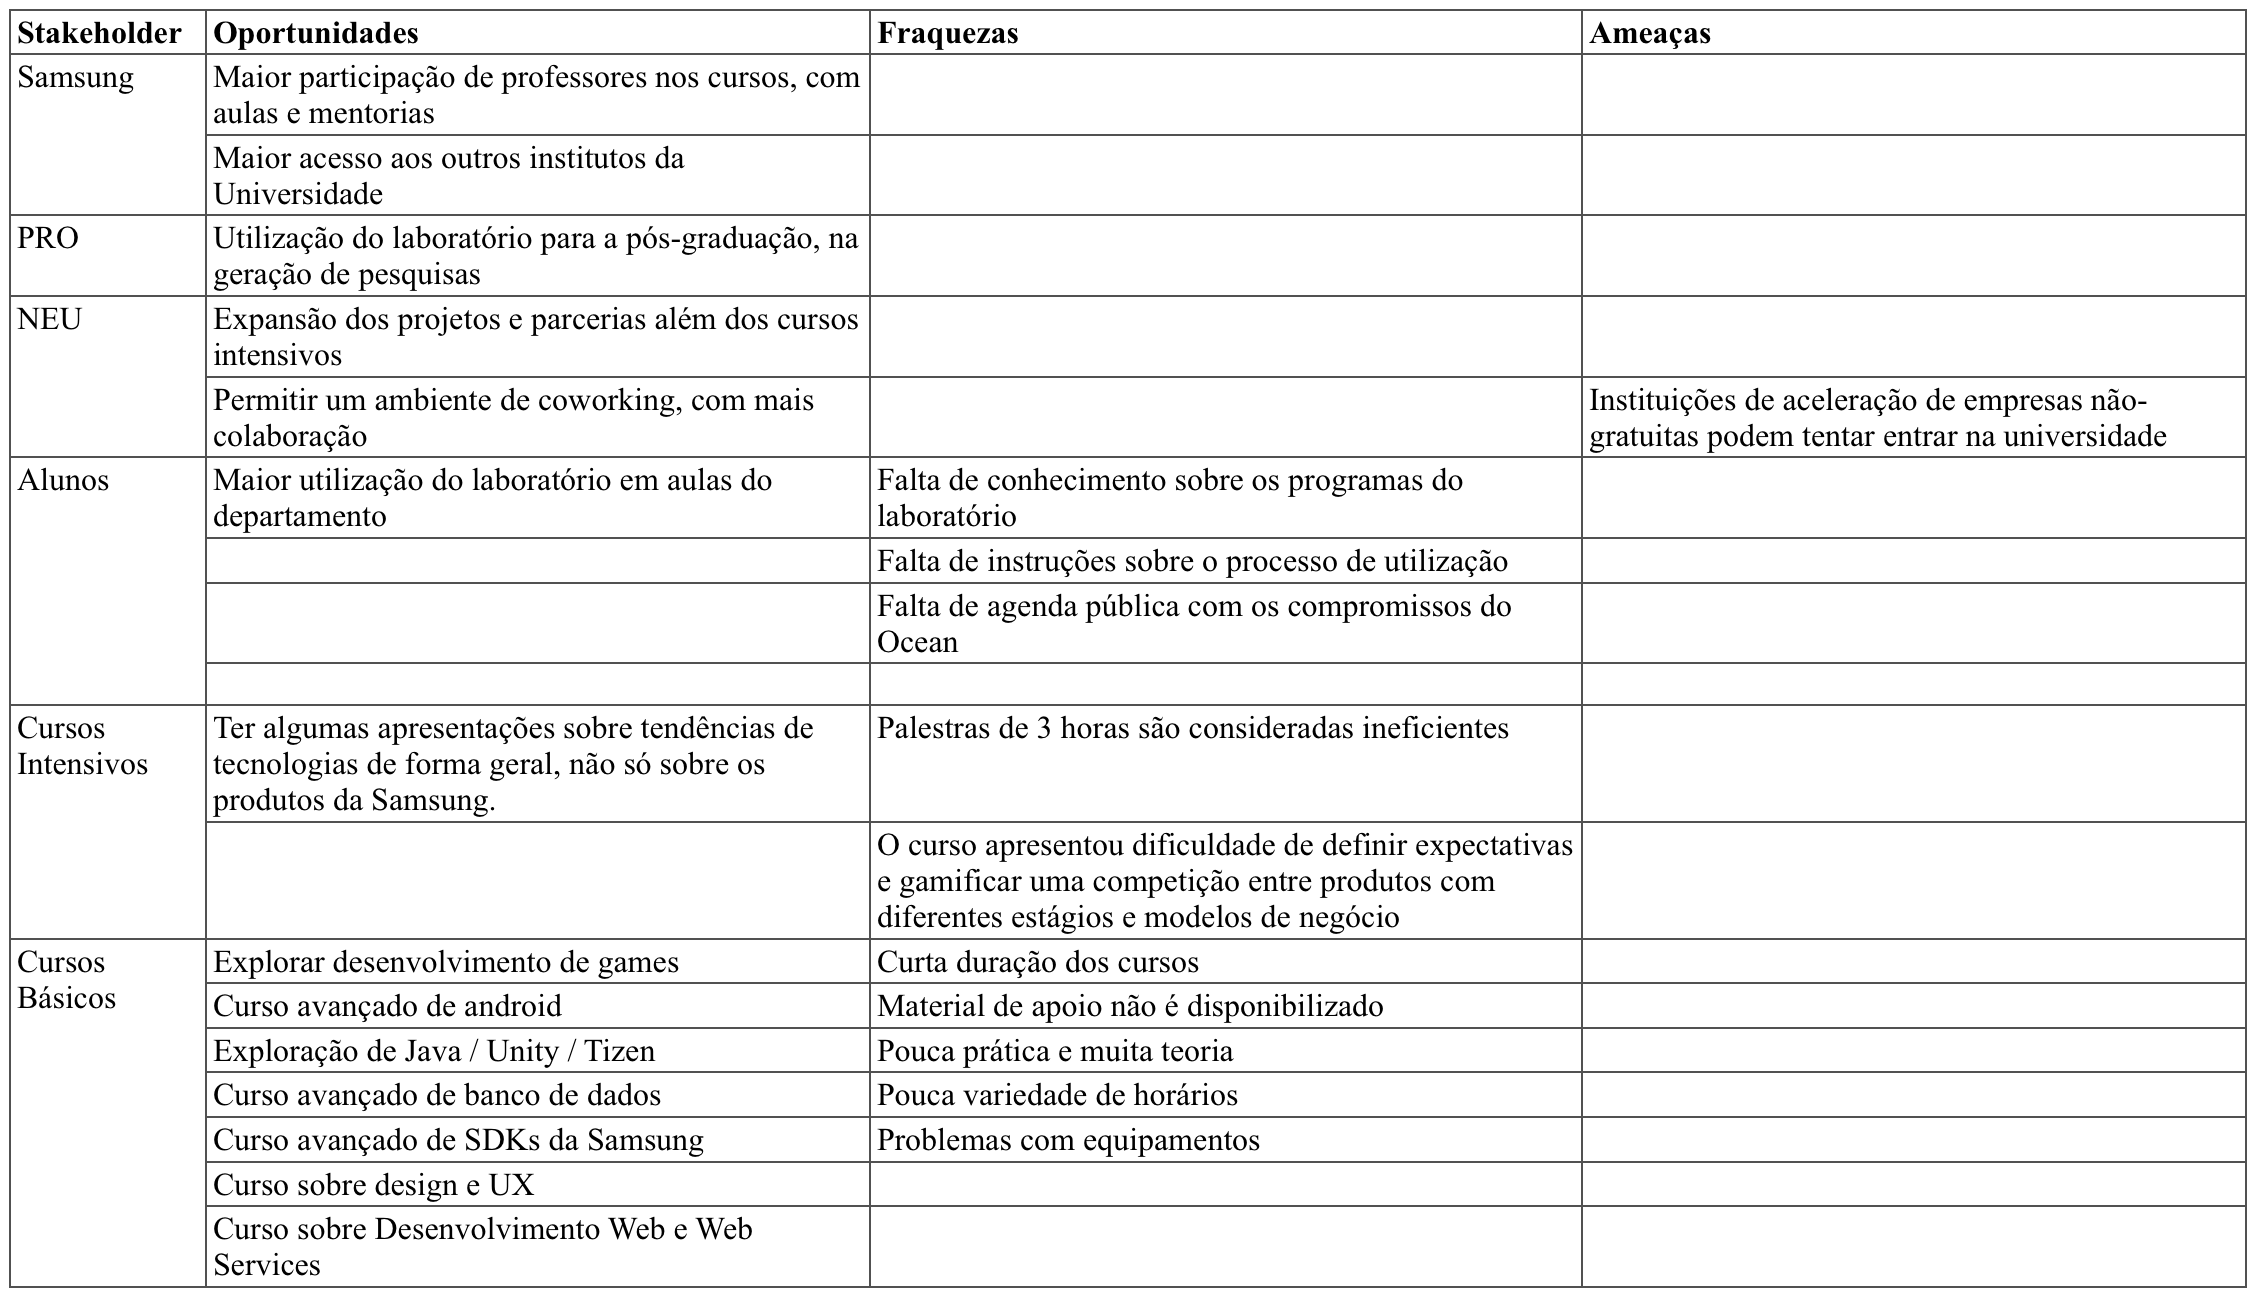
\includegraphics[scale=0.6]{img/oportunidadesfraquezasameacas}}
\label{fig:oportunidadesfraquezasameacas}
\caption* {Fonte: Elaborado pelo próprio autor}
\end{figure}

\end{landscape}
